%************************************************
\chapter{Equazioni conservative del moto}\label{chp:ConservazioneMoto}
%************************************************
Esistono due approcci alla descrizione del moto di un fluido all'interno di un determinato volume:
\begin{itemize}
\item Approccio Lagrangiano
\item Approccio Euleriano
\end{itemize}
\paragraph{Approccio Lagrangiano}
La descrizione lagrangiana di un flusso di un fluido traccia la posizione delle singole particelle dello stesso.
Il flusso può essere pensato come la composizione di un un numero finito di particelle di fluido che hanno: massa, momento, energia inerziale e altre proprietà. Dunque si può descrivere lo stato delle singole particelle a partire da equazioni per ognuna.
Ciò rende difficile sfruttare questo metodo per un'analisi pratica:
\begin{enumerate}
\item I fluidi sono composti da miliardi di molecole (particelle);
\item le interazioni tra le molecole sono difficili da descrivere analiticamente.
\end{enumerate} 
Questo approccio viene comunque usato in alcuni campi come: dinamica di spray, bolle e particelle; per l'accoppiamento dei metodi euleriani-lagrangiani.

\paragraph{Approccio Euleriano}
la descrizione euleriana di un fluido, viene definito un volume di controllo in cui il fluido scorre all'interno.
Si considera come le proprietà del fluido cambiano nel volume di controllo, che viene fissato nello spazio e nel tempo. Invece che seguire le singole particelle nello spazio.
Viene definito uno spazio di variabili che sono funzioni dello spazio e del tempo come:
\begin{description}
\item[Campo di velocità] $\textbf{V} = \textbf{V}(x, y, z, t)$
\item[Campo di pressione] $p = p(x, y, z, t)$
\item[Campo di densità] $\rho = \rho(x, y, z, t)$
\item[Campo di temperatura] $T = T(x, y, z, t)$
\item[\dots]
\end{description}
Resta necessario imporre una serie di condizioni di contorno affinché il sistema possa essere ben definito.

Alla figura \ref{fig:ModelliLagEul} vengono rappresentati i due modelli.

\begin{figure}
\centering
\subfloat[][\emph{Modello lagrangiano}\label{fig:Lagrangiano}]
{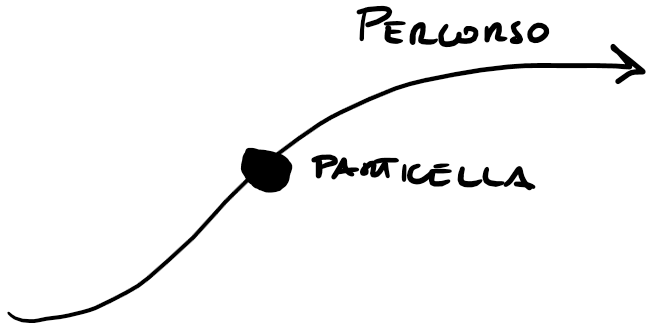
\includegraphics[width = 0.4\textwidth]{gfx/Lagrangiano}}\quad
\subfloat[][\emph{Modello Euleriano}\label{fig:Euleriano}]
{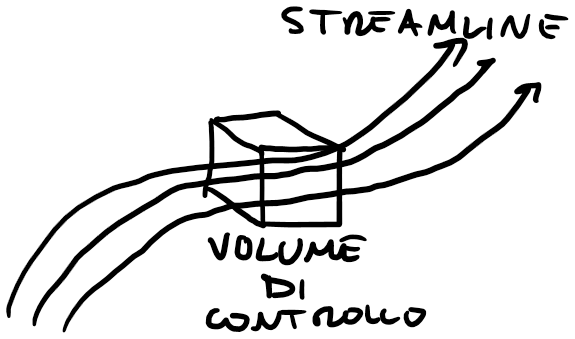
\includegraphics[width = 0.4\textwidth]{gfx/Euleriano}}
\caption{Esempi dei modelli di Lagrange ed Eulero}
\label{fig:ModelliLagEul}
\end{figure}

\section{Particelle di un fluido}
Il comportamento di un fluido è definito in termini macroscopici da%
\footnote{Vengono ignorate le notazioni $(x, y, z, t)$ per comodità, si ricorda che sono tutte funzioni di questi parametri.}
:
\begin{itemize}
\item Velocità $\textbf{u}$
\item Pressione $p$
\item Densità $\rho$
\item Temperatura $T$
\item Energia (cinetica) $E$, Entalpia $H$
\end{itemize}
Le proprietà risultano medie nel caso si considerino un numero sufficiente di particelle.
Un elemento fluido può essere pensato come il più piccolo volume per il quale la condizione di continuità è comunque valida.

\subsection{Derivate totali}
Considerando un fluido arbitrario, per una particella in moto nel fluido, questa sperimenta:
\begin{enumerate}
\item un cambiamento del fluido in funzione del tempo;
\item cambiamenti in base al fatto che più particelle si muovono in diverse direzioni nel fluido con diverse condizioni.
\end{enumerate}
La somma di queste due, per una caratteristica per unità di massa è chiamata come la derivata totale:
\begin{equation}
\frac{D\phi}{Dt} = \frac{\partial \phi}{\partial t} + V_x \frac{\partial \phi}{\partial x} + V_y \frac{\partial \phi}{\partial y} + V_z \frac{\partial \phi}{\partial z} = \frac{\partial \phi}{\partial t} + (\textbf{V} \cdot \nabla)\phi
\label{eqn:DerivataTotale}
\end{equation}
L'operatore \textbf{derivata totale}, $D/Dt$, fornisce la trasformazione tra il modello lagrangiano e quello euleriano.

Considerando l'accelerazione del fluido, può essere definita come:
\begin{equation}
\frac{D\mathbf{V}}{Dt} = \frac{\partial \mathbf{V}}{\partial t} + (\mathbf{V}\cdot \nabla) \mathbf{V}
\label{eqn:Accelerazione}
\end{equation}

dove:\\
\begin{tabular}{cl}
$\frac{\partial}{\partial t}$ & Derivata locale\\
$(\mathbf{V} \cdot \nabla) \mathbf{V}$ & Derivata di convezione\\
\end{tabular}\\

La derivata locale è diversa da zero solamente nel caso di flussi stazionari.
Mentre, la derivate di convezione è principalmente dovuta al fatto che le particelle sono in movimento.

Dunque, se la velocità del fluido è costante allora: l'accelerazione locale è nulla, allo stesso modo, l'accelerazione di convezione è sempre diversa da zero perché la particella si muove in altre posizioni caratterizzata dalla diversa velocità nel fluido.

Prendiamo come esempio il caso del flusso d'acqua dall'ugello, rappresentato in figura \ref{fig:EsempioAcqua}. 
Consideriamo per esempio l'approccio Euleriano sotto le seguenti ipotesi:
il flusso è stazionario nel caso in cui tutte le proprietà del flusso non cambiano in funzione del tempo.

\begin{figure}
\centering
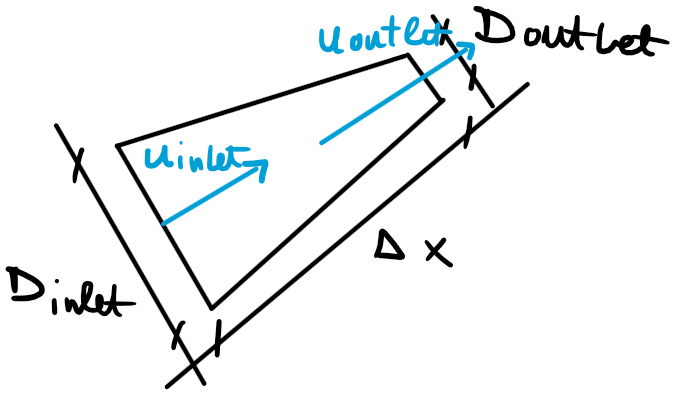
\includegraphics[width = 0.7\textwidth]{gfx/EsempioAcqua}
\caption{Esempio dell'ugello della canna dell'acqua}
\label{fig:EsempioAcqua}	
\end{figure}

Vale che la velocità all'uscita dell'ugello è più grande rispetto a quella di ingresso.
Perciò, il fluido deve accelerare all'interno del volume, anche se si è sotto l'ipotesi di stazionarietà.
Qui entra in gioco la derivata di convezione, questo parametro sarà sicuramente non nullo da cui i fenomeni di accelerazione.

Si evince che: secondo il modello euleriano, il sistema risulta stazionario. se invece si trasporta il tutto nel modello lagrangiano, ne risulta un'accelerazione delle particelle che entrano ad una data velocità ma escono ad una superiore.

\section{Conservazione della massa}
\begin{equation}
\frac{\partial \rho}{\partial t} + \nabla \cdot (\rho\mathbf{V}) = 0
\label{eqn:EquazioneConservazione}
\end{equation}

\begin{quote}
\emph{Il flusso in entrata e in uscita da un determinato volume varia al variare della massa compresa all'interno dello stesso volume di controllo.}
\end{quote}

\subsection{Funzione di flusso}
Le linee di corrente o \textbf{\eng{Streamlines}} soddisfano l'equazione di continuità e rappresentano su un piano cartesiano la funzione di flusso.

prendiamo il caso di un fluido bidimensionale incomprimibile sul piano x-y%
\footnote{$V_z = 0$ sia $V_x$ che $V_y$ non dipendono dalle componenti in $z$}.
L'equazione di continuità viene ridotta a $\frac{\partial V_x}{\partial x} + \frac{\partial V_y}{\partial y} = 0$.
La trasformazione di una variabile ci permette di riscrivere l'equazione in termini dipendenti da una sola variabile: la \textbf{funzione di flusso $\Psi$}:
\graffito{Il significato fisico della funzione $\Psi$ è che le curve della costante rappresentano le \eng{streamlines} del flusso.}
\begin{equation}
V_x = \frac{\partial \Psi}{\partial y} \qquad V_y = \frac{\partial \Psi}{\partial x}
\label{eqn:CambioVar}
\end{equation} 
Sostituendo nell'equazione di continuità:
\begin{equation}
\frac{\partial^2 \Psi}{\partial x \partial y} - \frac{\partial^2 \Psi}{\partial x \partial y} = 0
\label{eqn:StreamFunction}
\end{equation}

\begin{figure}
\centering
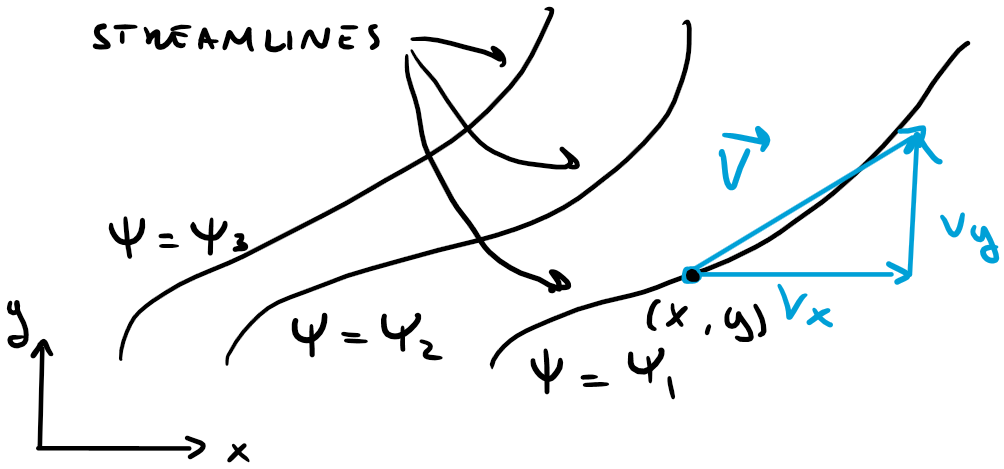
\includegraphics[width = \textwidth]{gfx/Streamlines}
\caption{Rappresentazione delle \eng{streamlines}}
\label{fig:Streamlines}
\end{figure}

Un'ulteriore considerazione deriva dal fatto che seguendo le ipotesi di:
\begin{itemize}
\item si assume che un fluido possa essere rapresentato tramite \eng{streamlines};
\item valga comunque la similitudine dei triangoli;
\end{itemize}
Allora si dimostra che:\\
\textit{La \eng{streamline} è una curva che è sempre istantaneamente tangente al vettore velocità locale}.

A partire dalla similitudine dei triangoli vale che (Vedi figura \ref{fig:Streamlines}):
\begin{equation}
\frac{dr}{V} = \frac{dx}{V_x} = \frac{dy}{V_y}
\label{eqn:SimTriangoli}
\end{equation}
Dalla \eqref{eqn:SimTriangoli} vale: $V_x dy = V_x dy$.
Sostituendo con la definizione della \eqref{eqn:CambioVar}, può essere scritta la:
\begin{equation}
\frac{\partial \Psi}{\partial y} dy + \frac{\partial \Psi}{\partial x} dx = 0
\end{equation}
Allora la variazione totale di $\Psi$ (in uno spazio infinitesimale $x+dx, y+dy$) vale%
\footnote{Si ricorda che la somma delle derivate parziali fatte rispetto alle variabili indipendenti è la derivata totale.}:
\begin{equation}
\frac{\partial \Psi}{\partial y} dy + \frac{\partial \Psi}{\partial x} dx = d\Psi
\end{equation}
Da cui deve essere che 
\begin{equation}
d\Psi = 0
\end{equation}
Questo significa che $\Psi = cost.$ lungo le \eng{streamlines}.

\graffito{Il significato fisico di questa affermazione è che: \textit{la differenza del valore di $\Psi$ tra due \eng{streamlines} è uguale al flusso di volume per la distanza tra le due linee}.}
Siccome, per definizione, alcun flusso può attraversare una \eng{streamline}, il fluido reste confinato tra le due stesse.
Ne segue che, per un flusso stazionario e incomprimibile bidimensionale, il flusso di volume $\dot{V}$ per unità di tempo tra due \eng{streamlines} deve essere costante (per garantire la validità dell'equazione di continuità).
Se due \eng{streamlines} si separano, la velocità media del flusso calerà uniformemente.

Analogamente a quanto visto fin ora, ovvero una descrizione delle \eng{streamlines} in coordinate cartesiane; la trattazione è del tutto equivalente per un sistema di riferimento in coordinate cilindriche.
A partire dalle stesse ipotesi, l'equazione di continuità può essere descritta come:
\begin{equation}
\frac{\partial (r V_r)}{\partial r} + \frac{\partial V_{\theta}}{\partial \theta} = 0
\end{equation}
Ora, la funzione di continuità viene comunque soddisfatta da una qualsiasi legge continua $\Psi = \Psi(r,\theta)$ dato che l'ordine di differenziazione è irrilevante.
Allora, per un fluido incomprimibile assisimmetrico (c'è simmetria nella rotazione dell'asse $z$) in assenza di vortici%
\footnote{$V_{\theta} = 0$ né $V_r$ né $V_z$ dipendono da $\theta$}, la funzione di continuità può essere descritta come
\begin{equation}
\frac{1}{r}\frac{\partial r V_r}{\partial r} + \frac{\partial V_z}{\partial z}  = 0
\end{equation}

\paragraph{Considerazioni}
Al di là della definizione di \eng{streamline} in qualsiasi sistema di riferimento, grazie all'osservazione di queste si può tracciare le linee di corrente soddisfacenti la conservazione della massa, permettendo di descrivere l'andamento del flusso all'interno del volume.
Vale anche:
\begin{description}
\item[\eng{streamlines} divergenti] $\Rightarrow$ velocità di flusso maggiore $\Rightarrow$ accelerazione delle particelle o flusso.
\item[\eng{streamlines} convergenti] $\Rightarrow$ Velocità di flusso minore $\Rightarrow$ decelerazione delle particelle o flusso.
\end{description}

\section{Conservazione del momento}
Per la trattazione della conservazione del momento da parte delle particelle di un fluido è necessario introdurre l'\textbf{equazione di Cauchy}.

\subsection{Equazione di Cauchy}
\begin{equation}
\rho \frac{D\mathbf{V}}{Dt} = \rho \vec{g} + \nabla \cdot \boldsymbol{\sigma}
\label{eqn:Cauchy}
\end{equation}
Dove viene definito $\boldsymbol{\sigma}$ come \textbf{Cauchy stress tensor}:
\begin{equation}
\boldsymbol{\sigma} = -p\mathbf{I} + \boldsymbol{\tau}
\label{eqn:StressTensorCauchy}
\end{equation}
Che scritto in forma matriciale diventa:
\begin{equation}
\underbrace{%
\begin{bmatrix}
\sigma_{xx} & \sigma_{xy} & \sigma_{xy} \\
\sigma_{yx} & \sigma_{yy} & \sigma_{yz} \\
\sigma_{zx} & \sigma_{zy} & \sigma_{zz}
\end{bmatrix}}_{= \boldsymbol{\sigma}} =%
\underbrace{%
\begin{bmatrix}
-p & 0 & 0 \\
0 & -p & 0 \\
0 & 0 & -p
\end{bmatrix}}_{\text{parte isotropica di } \boldsymbol{\sigma}} +%
\underbrace{%
\begin{bmatrix}
\tau_{xx} & \tau_{xy} & \tau_{xz} \\
\tau_{yx} & \tau_{yy} & \tau_{yz} \\
\tau_{zx} & \tau_{zy} & \tau_{zz} 
\end{bmatrix}}_{\text{parte anisotropa di} \boldsymbol{\sigma}}
\label{eqn:StressTensorCauchyMatrix}
\end{equation}
Per un fluido a riposo, l'unico sforzo in un elemento del fluido è la pressione idrostatica locale, la quale agisce uniformemente normale a qualsiasi superficie del fluido (componente isotropa di $\boldsymbol{\sigma}$).
Mentre, per un fluido in movimento, agisce comunque la componente isotropa. In più si aggiunge l'effetto dello sforzo viscoso $\boldsymbol{\tau}$ (componente anisotropa di $\boldsymbol{\sigma}$).
Tra l'altro, resta valido il fatto che lo sforzo viscoso è un effetto interno del fluido e non sulla superficie di controllo come accade per la componente isotropa.

Ora è necessario andare a descrivere che comportamento i fluidi abbiano in termini di componente anisotropa. Si rende necessario dividere i fluidi in base alla legge caratteristica di questo comportamento ovvero:
\begin{itemize}
\item fluidi newtoniani
\item fluidi non newtoniani
\end{itemize}

\subsubsection{Fluidi newtoniani}
I fluidi newtoniani sono tutti quei fluidi in cui lo sforzo viscoso è linearmente proporzionale alla deformazione del fluido.
In parole povere:
\begin{equation}
\boldsymbol{\tau} \propto \boldsymbol{\epsilon}
\end{equation}
Possiamo definire che la proporzionalità, assumendo che valga l'ipotesi di Stokes%
\footnote{Ovvero che il comportamento del fluido sia comparabile lungo i tre assi principali}:
\begin{equation}
\boldsymbol{\tau} = 2 \mu \boldsymbol{\epsilon} - \frac{2}{3} \mu \nabla \cdot \mathbf{V}
\label{eqn:NewtFluid}
\end{equation}
Nell'equazione \eqref{eqn:NewtFluid} viene aggiunto il parametro $\mu$ il quale indica la viscosità dinamica. Spesso si può trovare anche sotto forma di $\nu$ definito come $\nu = \mu / \rho$.
Si può legare la viscosità dinamica, in entrambe le sue forme, come: $\mu = f(T,p)$ ovvero che la viscosità dinamica dipende sia dalla temperatura che dalla pressione.
In particolare, si può dimostrare come dipenda fortemente dalle variazioni di temperatura e debolmente da quelle di pressione.
Resta importante capire che la viscosità dinamica è un fenomeno interno al fluido, qualunque esso sia, infatti si tratta della frizione tra i vari substrati del fluido.

\subsubsection{Fluidi non newtoniani}
Per questi fluidi non si può considerare la viscosità come costante, ma potrebbe variare in funzione dello sforzo.
Riprendendo i termini dell'equazione di Cauchy \eqref{eqn:StressTensorCauchy}:
\begin{equation}
\boldsymbol{\sigma} = \mu \dot{\gamma}
\label{eqn:NonNewtFluid}
\end{equation} 

\subsection{Equazione di Navier-Sockes}
\begin{equation}
\rho \frac{D\mathbf{V}}{Dt} = \rho \mathbf{g} - \nabla p + \mu \nabla^2\mathbf{V} + \frac{\mu}{3}\nabla(\nabla \cdot \mathbf{V})
\label{eqn:NavierStockes} 
\end{equation}
La quale può essere semplificata nel caso sussistano determinate condizioni:
\begin{description}
\item[Fluido incomprimibile] $(\nabla \cdot \mathbf{V}) = 0 $ allora l'equazione diventa:
\begin{equation}
\rho \frac{D\mathbf{V}}{Dt} = \rho \mathbf{g} - \nabla p + \mu \nabla^2\mathbf{V}
\end{equation}
\item[Fluido non viscido] si semplifica fino a:
\begin{equation}
\rho \frac{D\mathbf{V}}{Dt} = \rho \mathbf{g} - \nabla p
\end{equation}
\end{description}
Si definisce un fluido non viscido nel momento in cui le forze viscose sono trascurabili rispetto alle forze d'inerzia, gravitazionali e di pressione.
Ad esempio lo sono le zone del fluido ad alto numero di Reynolds.